%%%%%
%%%%% File name  : hw5_report.tex
%%%%% Author     : Yueh-Chou Lee
%%%%% Date       : April 31, 2020
%%%%%
%%
%%%
\documentclass[a4paper,11pt]{article}
\usepackage[top=2cm,bottom=2cm,outer=2cm,inner=2cm]{geometry}
\usepackage[utf8]{inputenc}
\usepackage[T1]{fontenc}
\usepackage{fontspec}
\usepackage{xeCJK}
\usepackage{amsfonts}
\usepackage{amsmath}
\usepackage{graphicx}
\usepackage{subfigure}
\usepackage{setspace}
\usepackage[explicit]{titlesec}
\usepackage{titlesec}
\usepackage{bibentry}
\usepackage[nottoc,numbib]{tocbibind} 
\usepackage{filecontents}
\usepackage{color}
\renewcommand{\baselinestretch}{2}
\setCJKmainfont{標楷體}


\title{Machine Learning Homework 5 Report}
\author{R06221012\hspace{0.2cm}數學所\hspace{0.2cm}李岳洲}
\date{April 31, 2020}

\begin{document}

\maketitle

\begin{enumerate}
	\item \textit{\textbf{從作業三可以發現,使用 CNN 的確有些好處,試繪出其 saliency maps,觀察模型在做 classification 時,是 focus 在圖片的哪些部份?}}\\

	\textbf{Discussion:}\\

		\begin{figure}[htp]
		    \begin{center}
		    		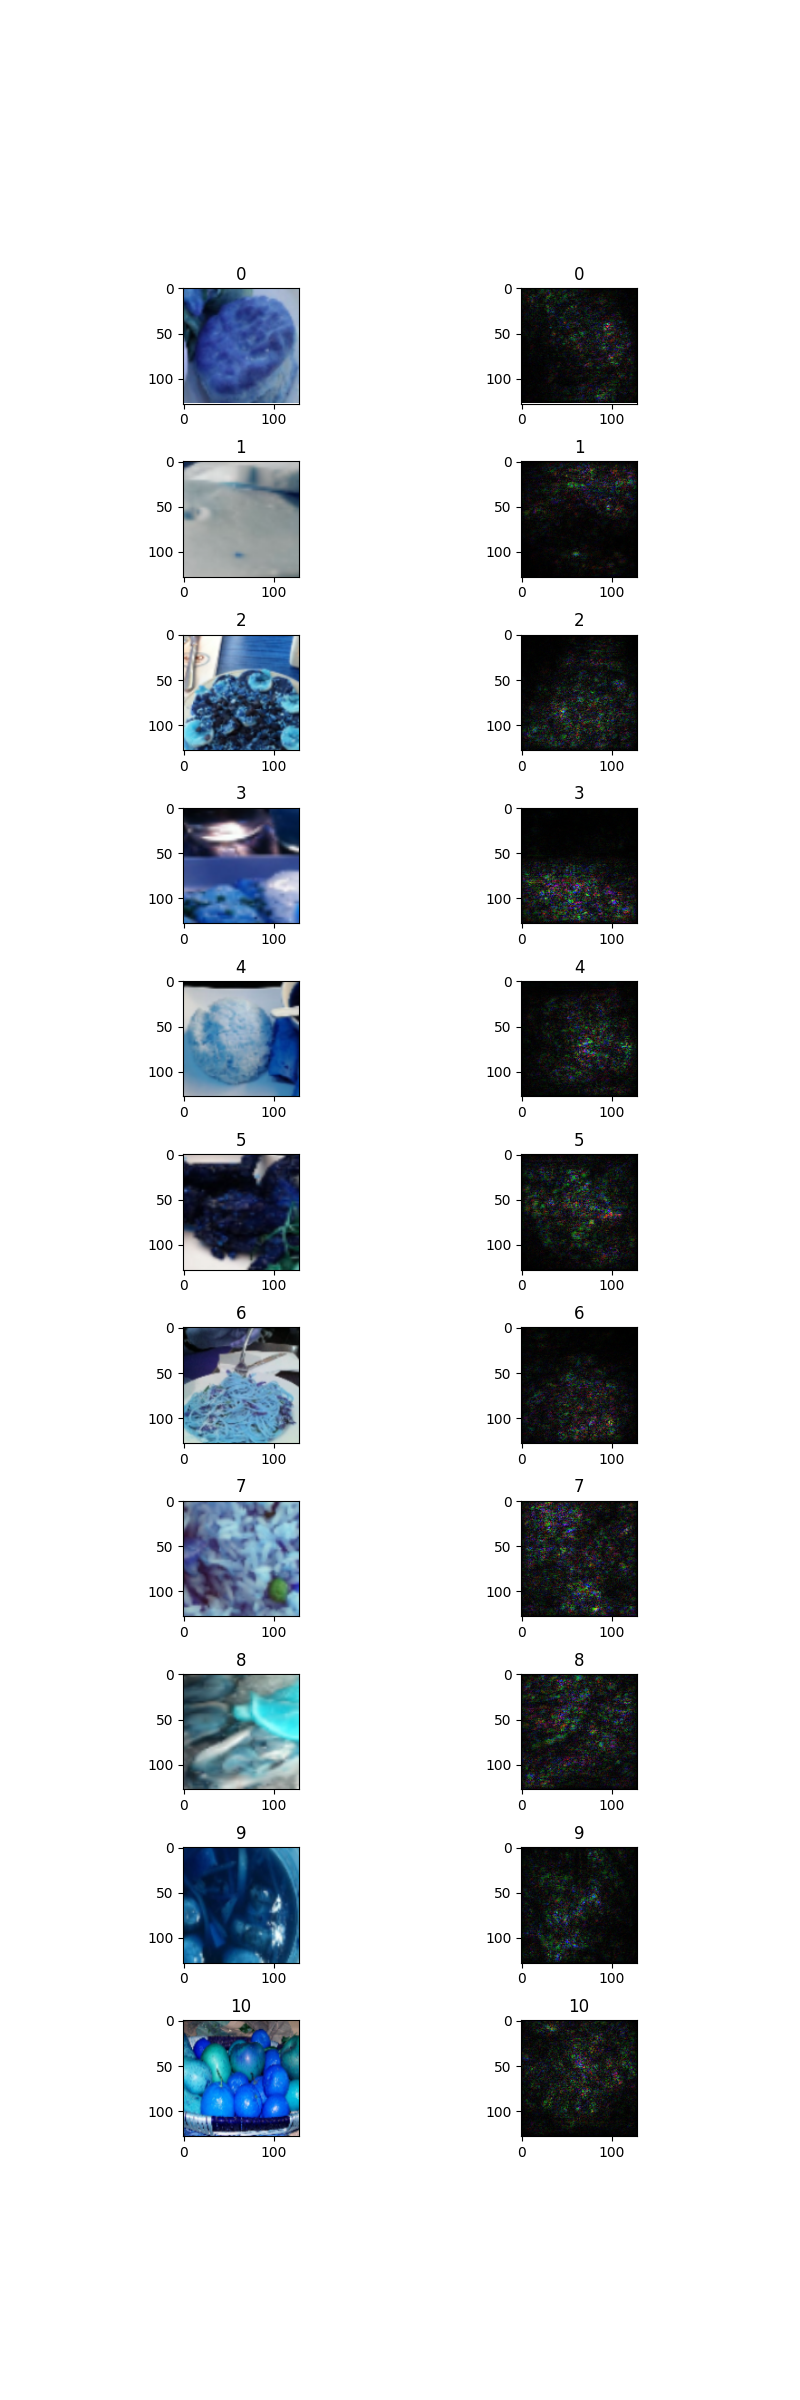
\includegraphics[scale=0.4]{./saliency_results.png}
		    	\caption{Saliency map}
		    \end{center}
		\end{figure}
\newpage

	\item \textit{\textbf{承上題,利用上課所提到的 gradient ascent 方法,觀察特定層的filter最容易被哪種圖片 activate 與觀察 filter 的 output。}}\\

	\textbf{Discussion:}\\

		\begin{figure}[htp]
		    \begin{center}
		    		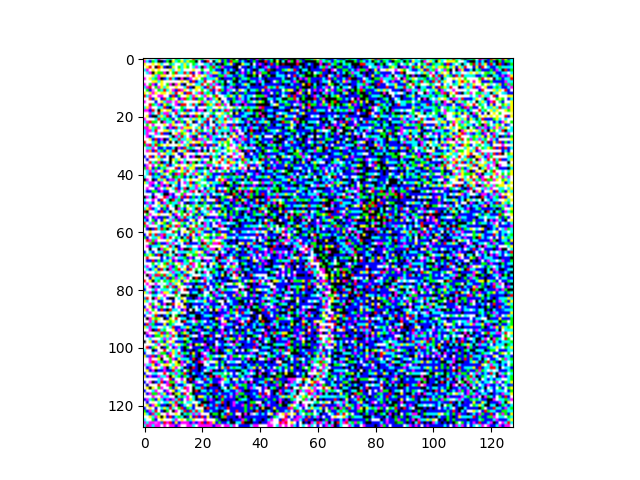
\includegraphics[scale=0.3]{./filter_layer_10.png}
		    	\caption{CNN layer 10}
		    \end{center}
		\end{figure}


		\begin{figure}[htp]
		    \begin{center}
		    		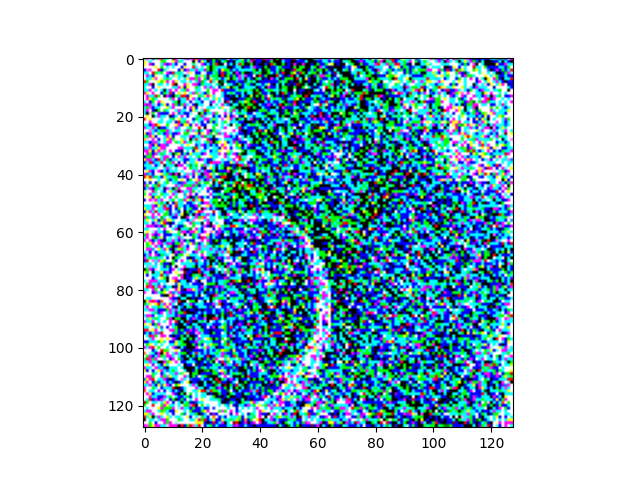
\includegraphics[scale=0.3]{./filter_layer_15.png}
		    	\caption{CNN layer 15}
		    \end{center}
		\end{figure}


		\begin{figure}[htp]
		    \begin{center}
		    		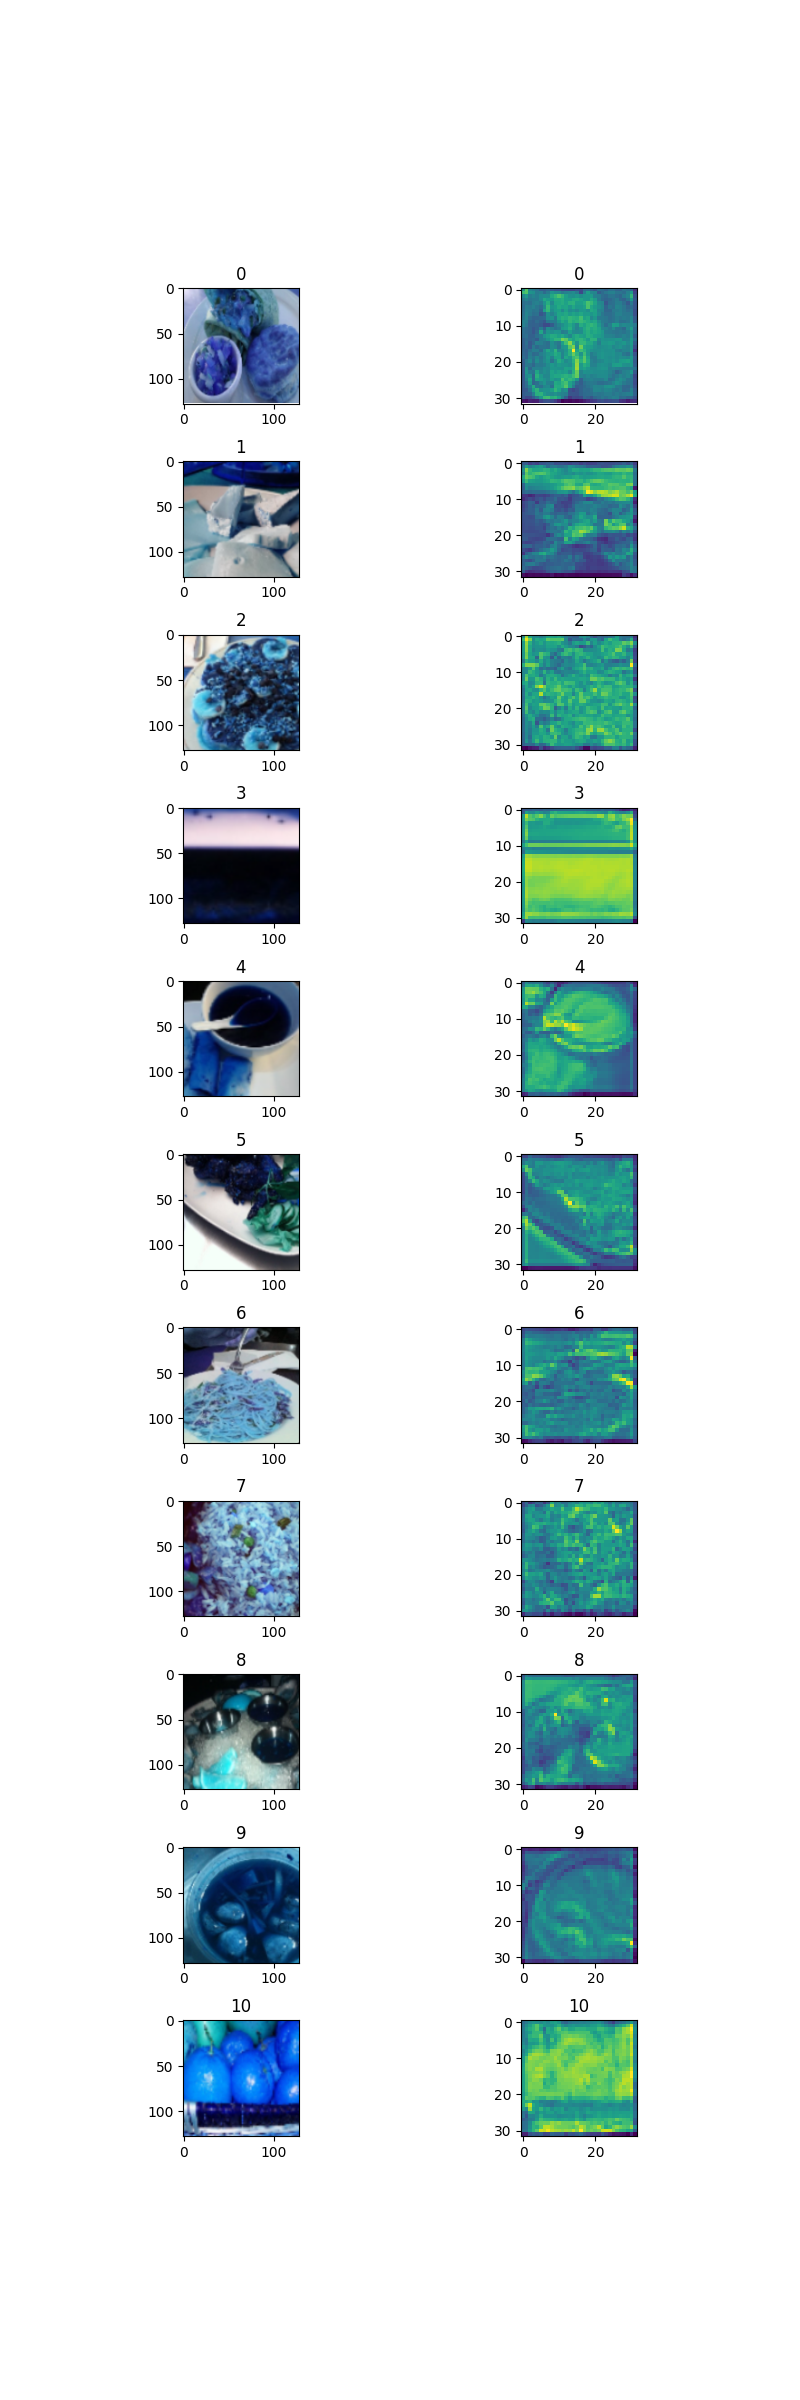
\includegraphics[scale=0.3]{./filter_layer_15_explaination_results.png}
		    	\caption{CNN layer 15 explaination}
		    \end{center}
		\end{figure}

\newpage

	\item \textit{\textbf{請使用 Lime 套件分析你的模型對於各種食物的判斷方式,並解釋為何你的模型在某些 label 表現得特別好。}}\\

	\textbf{Discussion:}

		\begin{figure}[htp]
		    \begin{center}
		    		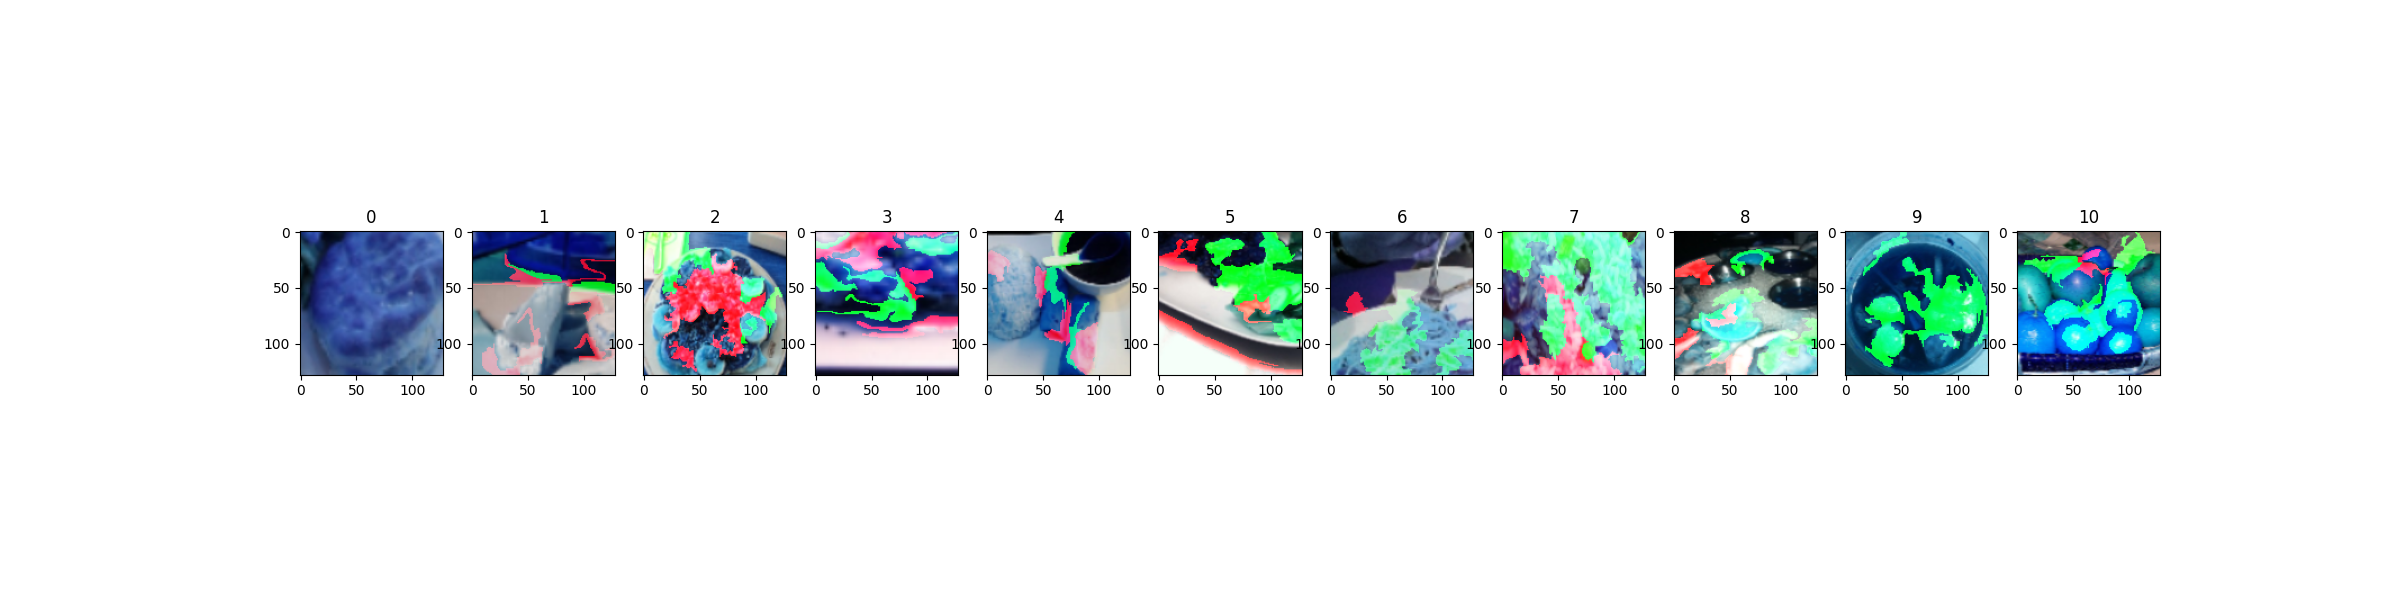
\includegraphics[scale=0.3]{./lime.png}
		    	\caption{SHAP}
		    \end{center}
		\end{figure}
	
	\item \textit{\textbf{請同學自行搜尋或參考上課曾提及的內容,實作任一種方式來觀察 CNN 模型的訓練,並說明你的實作方法及呈現 visualization 的結果。(請附上 reference)}}\\

	\textbf{Discuusion:}\\

\newpage

	\textbf{SHAP:}\\

		\begin{figure}[htp]
		    \begin{center}
		    		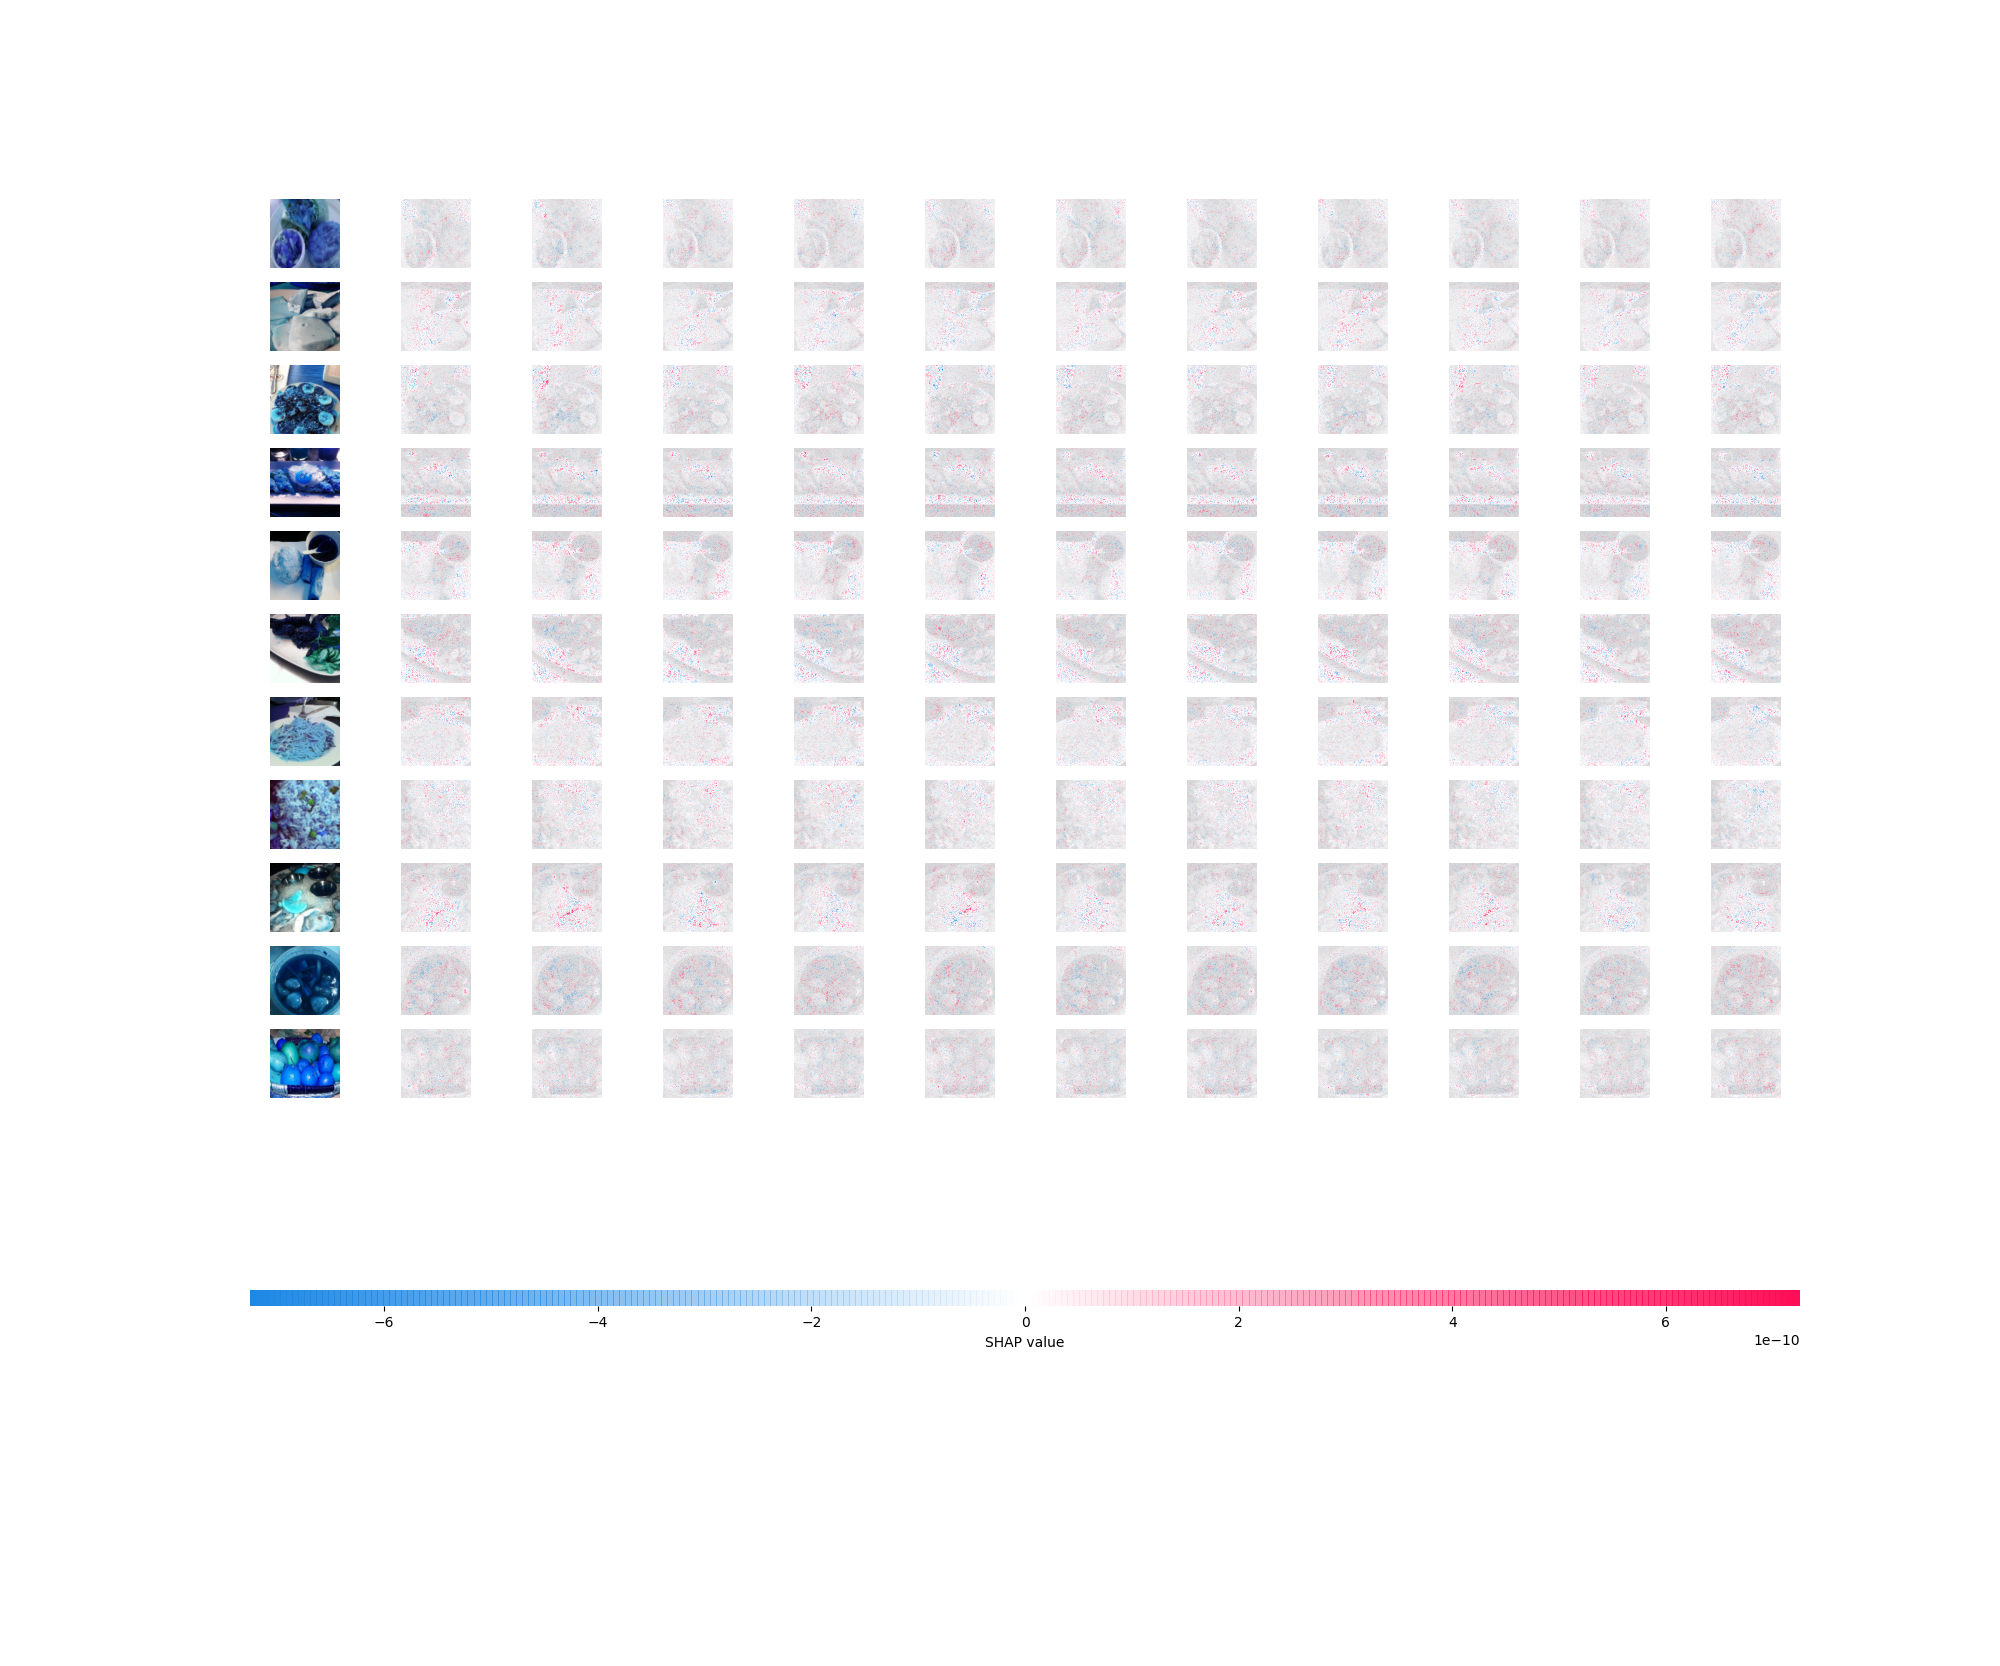
\includegraphics[scale=0.3]{./shap_results.png}
		    	\caption{SHAP}
		    \end{center}
		\end{figure}

\end{enumerate}
\end{document}